\documentclass[tikz,border=5pt]{standalone}
\usepackage{amsmath,amssymb}
\usepackage{newtxtext,newtxmath}
\usepackage{xcolor}
\usetikzlibrary{arrows.meta,calc}

% Lightened bright Morandi palette (35\% white blend)
\definecolor{MorandiCoral}{HTML}{EFAFA7}
\definecolor{MorandiApricot}{HTML}{F1C194}
\definecolor{MorandiMustard}{HTML}{E6CE8B}
\definecolor{MorandiSage}{HTML}{A8CAAA}
\definecolor{MorandiCyan}{HTML}{90C5C5}
\definecolor{MorandiSky}{HTML}{9BC0E2}
\definecolor{MorandiPeriwinkle}{HTML}{AAB1E0}
\definecolor{MorandiRose}{HTML}{CEA7C3}

\begin{document}
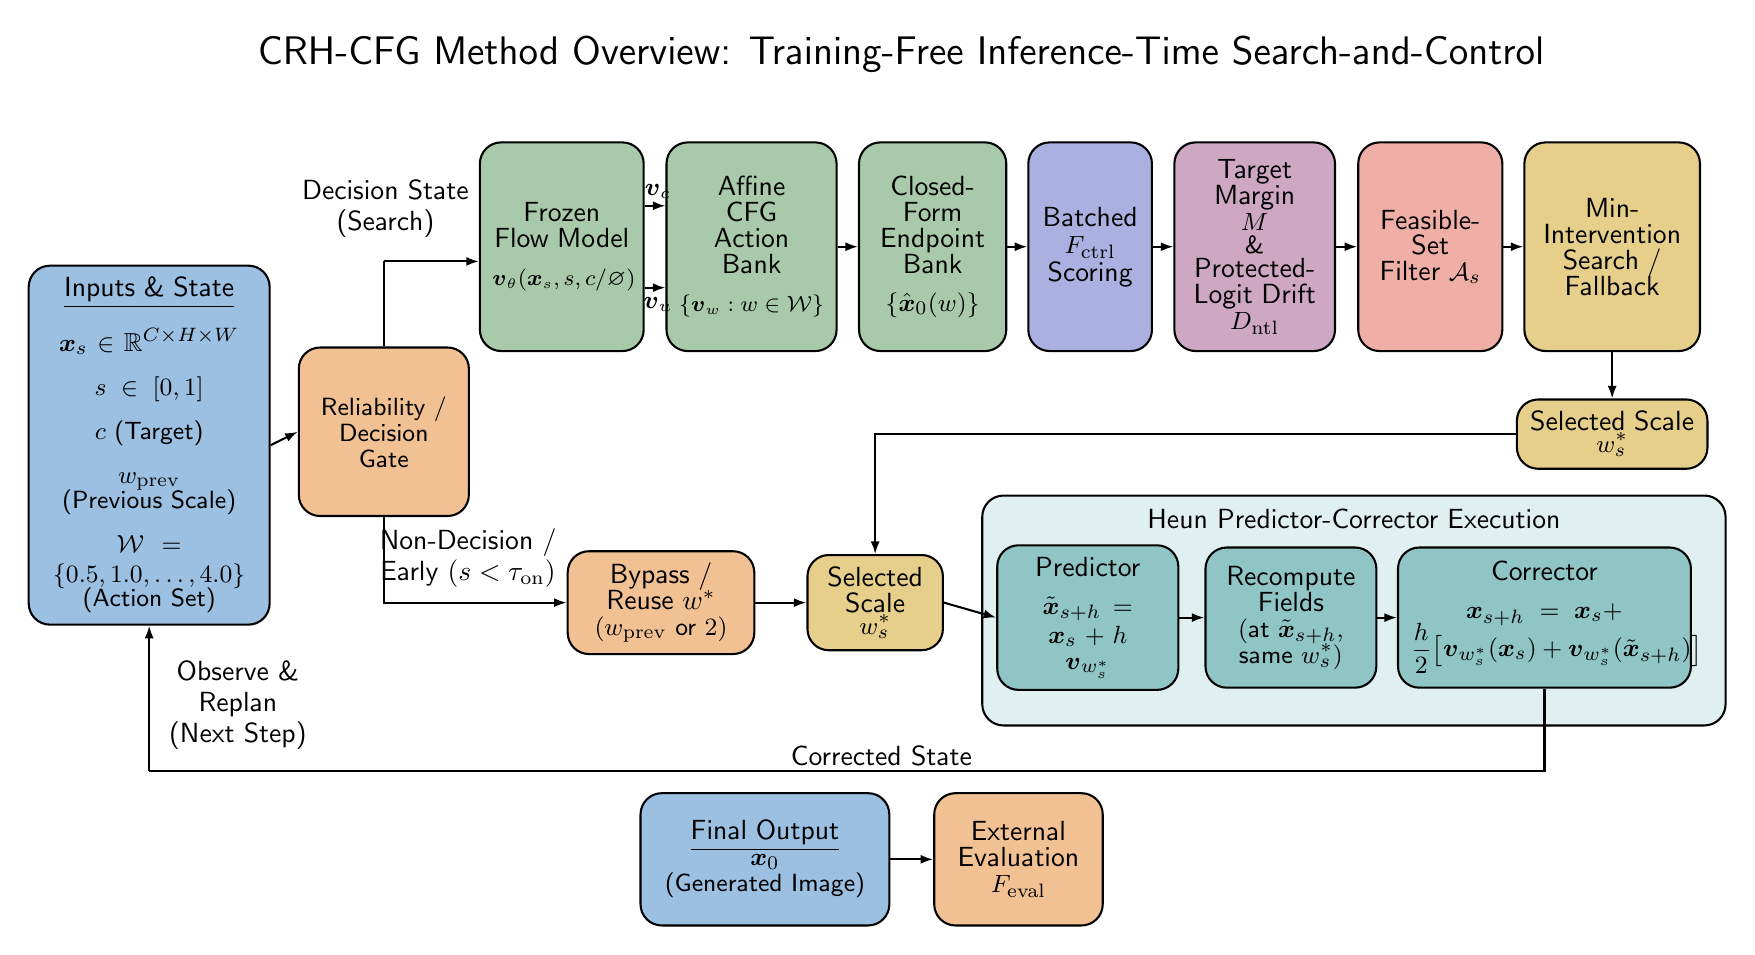
\begin{tikzpicture}[
  x=1cm,y=1cm,
  font=\sffamily\fontsize{9.4}{10.8}\selectfont,
  >={Latex[length=1.6mm,width=1.15mm]},
  flow/.style={-{Latex[length=1.6mm,width=1.15mm]},line width=0.75pt,draw=black},
  route/.style={line width=0.75pt,draw=black},
  box/.style={
    rounded corners=2.7mm,
    draw=black,
    line width=0.75pt,
    align=center,
    inner xsep=1.6mm,
    inner ysep=1.5mm,
    text=black
  },
  skybox/.style={box,fill=MorandiSky},
  sagebox/.style={box,fill=MorandiSage},
  periwinklebox/.style={box,fill=MorandiPeriwinkle},
  rosebox/.style={box,fill=MorandiRose},
  apricotbox/.style={box,fill=MorandiApricot},
  mustardbox/.style={box,fill=MorandiMustard},
  coralbox/.style={box,fill=MorandiCoral},
  cyanbox/.style={box,fill=MorandiCyan}
]

% Title
\node[font=\sffamily\fontsize{15.5}{18}\selectfont] at (11.15,11.62)
{CRH-CFG Method Overview: Training-Free Inference-Time Search-and-Control};

% Main blocks
\node[skybox,text width=2.74cm,minimum height=4.48cm] (input) at (1.60,6.66) {
  {\fontsize{10.4}{12}\selectfont\underline{Inputs \& State}}\\[2.2mm]
  $\boldsymbol{x}_s\in\mathbb{R}^{C\times H\times W}$\\[1.8mm]
  $s\in[0,1]$\\[1.8mm]
  $c$ (Target)\\[1.8mm]
  $w_{\mathrm{prev}}$\\[-0.7mm]
  (Previous Scale)\\[1.8mm]
  $\mathcal{W}=\{0.5,1.0,\ldots,4.0\}$\\[-0.7mm]
  (Action Set)
};

\node[apricotbox,text width=1.84cm,minimum height=2.14cm] (gate) at (4.58,6.83) {
  Reliability /\\[-0.5mm]
  Decision\\[-0.5mm]
  Gate
};

\node[sagebox,text width=1.76cm,minimum height=2.65cm] (frozen) at (6.84,9.18) {
  {\fontsize{10.2}{11.4}\selectfont Frozen}\\[-0.5mm]
  {\fontsize{10.2}{11.4}\selectfont Flow Model}\\[1mm]
  {\fontsize{7.8}{8.8}\selectfont$\boldsymbol{v}_{\theta}(\boldsymbol{x}_s,s,c/\varnothing)$}
};

\node[sagebox,text width=1.84cm,minimum height=2.65cm] (affine) at (9.25,9.18) {
  {\fontsize{10.2}{11.4}\selectfont Affine}\\[-0.5mm]
  {\fontsize{10.2}{11.4}\selectfont CFG}\\[-0.5mm]
  {\fontsize{10.2}{11.4}\selectfont Action}\\[-0.5mm]
  {\fontsize{10.2}{11.4}\selectfont Bank}\\[1mm]
  {\fontsize{7.6}{8.6}\selectfont\mbox{$\{\boldsymbol{v}_{w}:w\in\mathcal{W}\}$}}
};

\node[sagebox,text width=1.55cm,minimum height=2.65cm] (endpoint) at (11.55,9.18) {
  {\fontsize{10.2}{11.4}\selectfont Closed-}\\[-0.5mm]
  {\fontsize{10.2}{11.4}\selectfont Form}\\[-0.5mm]
  {\fontsize{10.2}{11.4}\selectfont Endpoint}\\[-0.5mm]
  {\fontsize{10.2}{11.4}\selectfont Bank}\\[1mm]
  $\{\hat{\boldsymbol{x}}_0(w)\}$
};

\node[periwinklebox,text width=1.25cm,minimum height=2.65cm] (score) at (13.55,9.18) {
  {\fontsize{10.2}{11.4}\selectfont Batched}\\[-0.3mm]
  $F_{\mathrm{ctrl}}$\\[-0.3mm]
  {\fontsize{10.2}{11.4}\selectfont Scoring}
};

\node[rosebox,text width=1.72cm,minimum height=2.65cm] (margin) at (15.64,9.18) {
  {\fontsize{10.2}{11.4}\selectfont Target}\\[-0.5mm]
  {\fontsize{10.2}{11.4}\selectfont Margin}\\[-0.5mm]
  $M$\\[-0.8mm]
  \&\\[-0.8mm]
  {\fontsize{10.2}{11.4}\selectfont Protected-}\\[-0.5mm]
  {\fontsize{10.2}{11.4}\selectfont Logit Drift}\\[-0.5mm]
  $D_{\mathrm{ntl}}$
};

\node[coralbox,text width=1.51cm,minimum height=2.65cm] (filter) at (17.87,9.18) {
  {\fontsize{10.2}{11.4}\selectfont Feasible-}\\[-0.5mm]
  {\fontsize{10.2}{11.4}\selectfont Set}\\[-0.5mm]
  {\fontsize{10.2}{11.4}\selectfont Filter} $\mathcal{A}_s$
};

\node[mustardbox,text width=1.91cm,minimum height=2.65cm] (search) at (20.18,9.18) {
  {\fontsize{10.2}{11.4}\selectfont Min-}\\[-0.5mm]
  {\fontsize{10.2}{11.4}\selectfont Intervention}\\[-0.5mm]
  {\fontsize{10.2}{11.4}\selectfont Search /}\\[-0.5mm]
  {\fontsize{10.2}{11.4}\selectfont Fallback}
};

\node[mustardbox,text width=2.10cm,minimum height=0.88cm] (selectedtop) at (20.18,6.80) {
  {\fontsize{10.0}{11.2}\selectfont Selected Scale}\\[-1mm]
  $w_s^{*}$
};

\node[apricotbox,text width=2.05cm,minimum height=1.24cm] (bypass) at (8.10,4.66) {
  {\fontsize{10.0}{11.2}\selectfont Bypass /}\\[-0.5mm]
  {\fontsize{10.0}{11.2}\selectfont Reuse $w^{*}$}\\[-0.5mm]
  $(w_{\mathrm{prev}}\ \text{or}\ 2)$
};

\node[mustardbox,text width=1.40cm,minimum height=1.12cm] (selectedmid) at (10.82,4.66) {
  {\fontsize{10.0}{11.2}\selectfont Selected}\\[-0.5mm]
  {\fontsize{10.0}{11.2}\selectfont Scale}\\[-1mm]
  $w_s^{*}$
};

% Heun predictor-corrector group
\draw[rounded corners=2.7mm,line width=0.75pt,fill=MorandiCyan!28!white]
  (12.18,3.10) rectangle (21.62,6.02);
\node[font=\sffamily\fontsize{10.4}{12}\selectfont] at (16.90,5.72)
{Heun Predictor-Corrector Execution};

\node[cyanbox,text width=1.98cm,minimum height=1.78cm] (predictor) at (13.52,4.47) {
  {\fontsize{10.0}{11.2}\selectfont Predictor}\\[1mm]
  $\tilde{\boldsymbol{x}}_{s+h}=\boldsymbol{x}_s+h$\\[-0.6mm]
  $\boldsymbol{v}_{w_s^{*}}$
};

\node[cyanbox,text width=1.85cm,minimum height=1.78cm] (recompute) at (16.10,4.47) {
  {\fontsize{10.0}{11.2}\selectfont Recompute}\\[-0.5mm]
  {\fontsize{10.0}{11.2}\selectfont Fields}\\[-0.5mm]
  $(\text{at }\tilde{\boldsymbol{x}}_{s+h},$\\[-0.5mm]
  $\text{same }w_s^{*})$
};

\node[cyanbox,text width=3.40cm,minimum height=1.78cm] (corrector) at (19.32,4.47) {
  {\fontsize{10.0}{11.2}\selectfont Corrector}\\[1mm]
  $\boldsymbol{x}_{s+h}=\boldsymbol{x}_s+$\\[-0.6mm]
  $\displaystyle\frac{h}{2}\!\left[\boldsymbol{v}_{w_s^{*}}(\boldsymbol{x}_s)+
  \boldsymbol{v}_{w_s^{*}}(\tilde{\boldsymbol{x}}_{s+h})\right]$
};

% Bottom blocks
\node[skybox,text width=2.84cm,minimum height=1.68cm] (final) at (9.42,1.40) {
  {\fontsize{10.3}{11.7}\selectfont\underline{Final Output}}\\[-0.5mm]
  $\boldsymbol{x}_0$\\[-0.5mm]
  (Generated Image)
};

\node[apricotbox,text width=1.82cm,minimum height=1.68cm] (eval) at (12.64,1.40) {
  {\fontsize{10.2}{11.5}\selectfont External}\\[-0.5mm]
  {\fontsize{10.2}{11.5}\selectfont Evaluation}\\[-0.5mm]
  $F_{\mathrm{eval}}$
};

% Main flow
\draw[flow] (input.east) -- (gate.west);

% Decision branch
\draw[route] (gate.north) -- ++(0,1.08) coordinate (decisionbend);
\draw[flow] (decisionbend) -- (frozen.west |- decisionbend);
\node[align=center,font=\sffamily\fontsize{10.0}{11.4}\selectfont] at (4.60,9.66)
{Decision State\\(Search)};

% Conditional and unconditional velocities
\draw[flow] ($(frozen.east)+(0,0.52)$) -- ($(affine.west)+(0,0.52)$);
\node[font=\sffamily\fontsize{8.7}{9.5}\selectfont] at (8.06,9.88) {$\boldsymbol{v}_c$};
\draw[flow] ($(frozen.east)+(0,-0.52)$) -- ($(affine.west)+(0,-0.52)$);
\node[font=\sffamily\fontsize{8.7}{9.5}\selectfont] at (8.06,8.45) {$\boldsymbol{v}_u$};

\draw[flow] (affine.east) -- (endpoint.west);
\draw[flow] (endpoint.east) -- (score.west);
\draw[flow] (score.east) -- (margin.west);
\draw[flow] (margin.east) -- (filter.west);
\draw[flow] (filter.east) -- (search.west);
\draw[flow] (search.south) -- (selectedtop.north);

% Search result routed back to execution scale
\draw[route] (selectedtop.west) -- (10.82,6.80) -- (10.82,5.36);
\draw[flow] (10.82,5.36) -- (selectedmid.north);

% Non-decision / early branch
\draw[route] (gate.south) -- (4.58,4.66) -- (6.78,4.66);
\draw[flow] (6.78,4.66) -- (bypass.west);
\node[align=center,font=\sffamily\fontsize{9.8}{11.2}\selectfont,anchor=south] at (5.65,4.73)
{Non-Decision /\\Early $(s<\tau_{\mathrm{on}})$};

\draw[flow] (bypass.east) -- (selectedmid.west);
\draw[flow] (selectedmid.east) -- (predictor.west);
\draw[flow] (predictor.east) -- (recompute.west);
\draw[flow] (recompute.east) -- (corrector.west);

% Corrected-state feedback loop
\draw[route] (corrector.south) -- (19.32,2.52) -- (1.60,2.52);
\draw[flow] (1.60,2.52) -- (input.south);
\node[font=\sffamily\fontsize{10.0}{11.4}\selectfont] at (10.90,2.72) {Corrected State};
\node[align=center,font=\sffamily\fontsize{9.8}{11.2}\selectfont,anchor=west] at (1.73,3.35)
{Observe \&\\Replan\\(Next Step)};

% Final output to evaluation
\draw[flow] (final.east) -- (eval.west);

\end{tikzpicture}
\end{document}
